\documentclass[11pt]{article}
\usepackage{datetime}
\usepackage{color,array,graphics}
\usepackage{enumerate}
\usepackage[pdftex, colorlinks, linkcolor=red,citecolor=red,urlcolor=blue]{hyperref}
\usepackage{ulem}

\setlength{\parindent}{0cm}

\setlength{\parskip}{0.3cm plus4mm minus3mm}

\textwidth  6.5in
\oddsidemargin +0.0in
\evensidemargin +0.0in
\textheight 9.0in
\topmargin -0.5in

\usepackage{upquote,textcomp}
\usepackage{amssymb,amsmath,amsfonts,amsthm}
\usepackage{graphicx}
\usepackage{multicol}

\usepackage{tikz}
\usetikzlibrary{automata,positioning}
\usepackage{tikz-qtree}


\newcommand{\vect}[1]{{\bf #1}}                 %for bold chars
\newcommand{\vecg}[1]{\mbox{\boldmath $ #1 $}}  %for bold greek chars
\newcommand{\matx}[1]{{\bf #1}}

\def\OR{\vee}
\def\AND{\wedge}
\def\imp{\rightarrow}
\def\math#1{$#1$}

\DeclareSymbolFont{AMSb}{U}{msb}{m}{n}
\DeclareMathSymbol{\N}{\mathbin}{AMSb}{"4E}
\DeclareMathSymbol{\Z}{\mathbin}{AMSb}{"5A}
\DeclareMathSymbol{\R}{\mathbin}{AMSb}{"52}
\DeclareMathSymbol{\Q}{\mathbin}{AMSb}{"51}
\DeclareMathSymbol{\I}{\mathbin}{AMSb}{"49}
\DeclareMathSymbol{\C}{\mathbin}{AMSb}{"43}

\begin{document}
\thispagestyle{empty}

\begin{center}
\large
\textbf{CSCI 2200 --- Foundations of Computer Science (FoCS) \\
Homework 5 (document version 1.0)}
\end{center}

\section*{Overview}
\begin{itemize}
\item This homework is due by 11:59PM on Thursday, December~7
\item You may work on this homework in a group of up to four students;
  unlike recitation problem sets,
  \textbf{your teammates may be in any section}
\item You may use at most \textbf{three} late days on this assignment
\item Please start this homework early and ask questions during
  office hours and at your November~1 recitation section;
  also ask questions on the Discussion Forum
\item Please be concise in your written answers;
  even if your solution is correct, if it is not well-presented,
  you may still lose points
\item You can type or hand-write (or both) your solutions
  to the required graded problems below;
  \textbf{all work must be organized in one PDF that lists
  all teammate names}
\item You are strongly encouraged to use LaTeX, in particular for
  mathematical symbols;
  see the corresponding \verb+hw5.tex+ file as a starting point
  and example
\end{itemize}

\newpage
\section*{Warm-up exercises}
The problems below are good practice problems to work on.
Do not submit these as part of your homework submission.
\textbf{These are ungraded problems.}

\begin{multicols}{2}
\begin{itemize}

\item \textbf{Problem 13.42.}
\item \textbf{Problem 13.46.}
\item \textbf{Problem 13.55.}
\item \textbf{Problem 13.58.}
\item \textbf{Problem 14.1.}
\item \textbf{Problem 14.2.}
\item \textbf{Problem 14.18.}
\item \textbf{Problem 14.34.}
\item \textbf{Problem 14.48.}
\item \textbf{Problem 14.63(g).}
\item \textbf{Problem 15.6.}
\item \textbf{Problem 15.18.}
\item \textbf{Problem 15.33.}
\item \textbf{Problem 15.35.}
\item \textbf{Problem 15.46.}
\item \textbf{Problem 16.26.}
\item \textbf{Problem 24.2.}
\item \textbf{Problem 24.3.}
\item \textbf{Problem 24.9.}
\item \textbf{Problem 24.11(a-e,g,i-v,x-z).}

\end{itemize}
\end{multicols}

\section*{Graded problems}
The problems below are required and will be graded.
\begin{itemize}

\item \textbf{*Problem 13.50.}
\item \textbf{*Problem 14.15(b-c).}  % PS8
\item \textbf{*Problem 14.19.}
\item \textbf{*Problem 15.12.}
\item \textbf{*Problem 15.32.}
\item \textbf{*Problem 24.11(f,h,w).}
\item \textbf{*Problem 25.7.}

\end{itemize}

As you might not have the required textbook yet,
all of the above problems (both graded and ungraded)
are transcribed in the pages that follow.

Graded problems are noted with an asterisk~(*).

If any typos exist below, please use the textbook description.

\newpage
\begin{itemize}

\item \textbf{Problem 13.42.}
To determine if a graph $G$ with 50 vertices is 3-colorable,
you test all possible 3-colorings.
Your computer checks a million 3-colorings per second.
Estimate how long it is going to take, in the worst case.

\vspace{0.2in}

\item \textbf{*Problem 13.50.}
How many 7-digit phone-numbers are non-decreasing
(each digit is not less than the previous one.)

\vspace{0.2in}

\item \textbf{Problem 13.55.}
In Example 13.3 on page 186, the King and Queen occupy different rows and columns.
If we relax that restriction, how many positions are possible?
Here are two arguments.
\begin{enumerate}[(i)]
\item There are 64 choices for the King and then 63 for the Queen.
  The product rule gives $64\times63=4032$ positions.
\item We count the sequences $c_Kr_Kc_Qr_Q$ as in Example~13.3, but now without
  the restriction that $c_Q\ne c_K$ and $r_Q\ne r_K$.
  By the product rule there are $8\times8\times8\times8=4096$ positions.
\end{enumerate}
Which reasoning is correct?
What is wrong in the other reasoning?
How are the two answers related?

\vspace{0.2in}

\item \textbf{Problem 13.58.}
List the 2 and 3 element subsets of $\{1,2,3,4,5\}$.
Pair each 2-subset with its complement (a 3-subset) to verify
that there are an equal number of 2 and 3-subsets.

\vspace{0.2in}

\item \textbf{Problem 14.1.}
How many different words can you form using the letters:
(a)~\textsc{abc} (b)~\textsc{aaa} (c)~\textsc{aardvark}?

\vspace{0.2in}

\item \textbf{Problem 14.2.}
How many different words can you form using the letters:
(a)~\textsc{rearrange} (b)~\textsc{bookkeeper} (c)~\textsc{discrete}?
(d)~\textsc{parallel} (e)~\textsc{success} (f)~\textsc{mississippi}?

\vspace{0.2in}

\item \textbf{*Problem 14.15(b-c).}  % PS8
Consider the binary strings consisting of 10~bits.

\begin{enumerate}[(a)]
\setcounter{enumi}{1}
\item How many contain (i) 5 or more consecutive 1's (ii)~5 or more consecutive 0's?
\item How many contain 5 or more consecutive 0's or 5 or more consecutive 1's?
\end{enumerate}

\vspace{0.2in}

\item \textbf{Problem 14.18.}
How many 8-bit sequences
(a)~begin or end in 1?
(b)~begin in 1 or have 101 starting at position 4?

\vspace{0.2in}

\item \textbf{*Problem 14.19.}
A 5-card poker hand is monochromatic if all cards are the same color;
it is a flush if all cards are the same suit.
How many hands are either a flush or monochromatic?

\textbf{Determine Number of Flush Hands}

There are 4 suits in a standard deck, with each suit having 13 cards

So within each suit, there are $\binom{13}{5}$ ways to choose 5 cards of that suit

So the number of flush hands = $4 * \binom{13}{5} = 4 * \frac{13!}{5!(13-5)!} = 4 * \frac{13!}{5!(8!)} = 4 * 1287 = \boxed{5148}$ 

\vspace*{0.1in}

\textbf{Determine number of monochromatic hands}

There are two colors in a standard deck of cards, red or black, with each color having 26 cards

So for each color, there are $\binom{26}{5}$ ways to choose 5 cards.

So the number of monochromatic hands = $2 * \binom{26}{5} = 2 * \frac{26!}{5!(26-5)!} = 2 * \frac{26!}{5!(21!)} = 2 * 65780 = \boxed{131560}$

\textbf{Number of cards either Flush or Monochromatic}

$5148 + 131560 = \boxed{136708}$

\vspace{0.2in}

\item \textbf{Problem 14.34.}
Consider all permutations of $\{1,2,3,4,5,6\}$.
A permutation is good if any of the sub-sequences 12, 23, or 56 appear.
How many good permutations are there?

\vspace{0.2in}

\item \textbf{Problem 14.48.}
ID-card numbers at a school start with an uppercase letter,
followed by a 2-bit binary string followed by another uppercase letter
followed by two decimal digits, e.g.,~$J01E38$.
\begin{enumerate}[(a)]
\item How many possible ID-card numbers are there?
\item 40,000 students get IDs.
  At least how many of the student IDs must satisfy each criterion:
  (i)~Have the same first letter?
  (ii)~Have the same first letter and last digit?
  (iii)~Start with~$J$?
\end{enumerate}

\vspace{0.2in}

\item \textbf{Problem 14.63(g).}
Here are some counting problems on graphs to challenge you.
\begin{enumerate}[(a)]
\setcounter{enumi}{6}
\item How many Hamiltonian cycles are in $K_{n,n}$?
  [Hint: a Hamiltonian cycle is a cycle on graph $G=(V,E)$ that
  starts and ends at vertex~$v_0\in V$,
  visiting each vertex in set $V-\{v_0\}$ (i.e.,~all other vertices)
  exactly once.]
\end{enumerate}

\vspace{0.2in}

\item \textbf{Problem 15.6.}
You roll a pair of fair dice.
Compute these probabilities:
\begin{multicols}{2}
\begin{enumerate}[(a)]
\item $\mathcal{P}[$sum exceeds 6$]$
\item $\mathcal{P}[$sum does not exceed 6$]$
\item $\mathcal{P}[$sum is even$]$
\item $\mathcal{P}[$sum is not even$]$
\item $\mathcal{P}[$sum exceeds 6 \textsc{and} is even$]$
\item $\mathcal{P}[$sum exceeds 6 \textsc{and} is not even$]$
\item $\mathcal{P}[$sum does not exceed 6 \textsc{and} is not even$]$
\item $\mathcal{P}[$sum exceeds 6 \textsc{or} is even$]$
\item $\mathcal{P}[$sum does not exceed 6 \textsc{or} is even$]$
\item $\mathcal{P}[$sum exceeds 6 \textsc{or} is not even$]$
\end{enumerate}
\end{multicols}

\newpage

\item \textbf{*Problem 15.12.}
Roll a 6-sided die 5 times.
What is the probability:
(a)~some number repeats
(b)~you get no sixes?

\subsection*{(a)}

Since there are 6 possible outcomes on each roll, the total number of outcomes when rolling die 5 times is $6^5 = 7776$. To have no repeats in 5 rolls, the first roll can be any number(6 options), the second roll can be any number except the first(5 options), and so on. This gives us $6 * 5*4*3*2 = 6! = 720$ ways to roll the dice without any repeats. So the probability of no repeats is $\frac{720}{7776}$

We can then subtract that from 1 to get the probability of at least one repeat. 

$1 - \frac{720}{7776} = \frac{7056}{7776} = 0.9074$, \textbf{So there is a 90.74\% chance that some number repeats}

\subsection*{(b)}

Using Binoimal Distribution

p - probability of getting 6 in a single roll - $\frac{1}{6}$

q = probability of not getting 6 in a single roll - $\frac{5}{6}$

n = number of rolls = 5

We don't want to get any 6s, so x is 0

Plug in

$P_0 = \binom{5}{0} * (\frac{1}{6})^0*(\frac{5}{6})^5 = 1 * 1 * (\frac{5}{6})^5 = (\frac{5}{6})^5 = 0.4019$

\textbf{There is a 40.19\% chance of not rolling a six in any of the 5 rolls}




\vspace{0.2in}

\item \textbf{Problem 15.18.}
A bag has 2 blue, 2 red, 2 green, and 2 pink balls.
You randomly pick 4 balls.
What is the probability that the number of different colors you get is (a)~4 (b)~3 (c)~2 (d)~1?

Repeat your calculations when you pick with replacement: after you pick each ball you
replace it back into the bag.

\vspace{0.2in}

\item \textbf{*Problem 15.32.}
Draw two cards randomly from a 52-card deck.
Compute the probabilities:
(a)~The first is a $K$ and the second a picture card ($A,K,Q,J$).
(b)~At least one card is a picture card.

\vspace{0.2in}

\item \textbf{Problem 15.33.}
Draw two cards randomly from a 52-card deck.
Compute the probabilities:
(a)~Both are $\spadesuit$.
(b)~One is $\spadesuit$.
(c)~One is $\spadesuit$ and one is $\heartsuit$.
(d)~One is $\spadesuit$ or one is $\heartsuit$.

\newpage

\item \textbf{Problem 15.35.}
Eight pawns are placed randomly on different squares of a chessboard.
\begin{enumerate}[(a)]
\item Compute the probability they are in a straight line (including diagonals).
\item Compute the probability no two are in the same row or column.
\end{enumerate}

\vspace{0.2in}

%\item \textbf{Problem 15.46.}
%
%\vspace{0.2in}

\item \textbf{Problem 16.26.}
Randomly draw 5 cards from a 52-card deck and reveal one.
Compute the probability of two aces if the revealed card is:
(a)~$\heartsuit A$
(b)~an Ace
(c)~$\heartsuit K$
(d)~not an Ace.

\vspace{0.2in}

\begin{multicols}{2}
\item \textbf{Problem 24.2.}
For the finite automaton on the right:
\begin{enumerate}[(a)]
\item What is the start state?
  What is the set of accept (i.e.,~final) states?
\item What sequence of states are followed for input 0011?
\item Give all strings of length at most 6 accepted by the machine.
\item Give the conditions on a general automaton $M$ under which $\varepsilon\in\mathcal{L}(M)$.
\end{enumerate}
\begin{center}
\end{center}
\begin{verbatim}


\end{verbatim}
\end{multicols}

\vspace{0.2in}

\item \textbf{Problem 24.3.}
Describe in words the language accepted by each automaton, and also give a regular expression.
\begin{center}
\end{center}

\vspace{0.2in}

\item \textbf{Problem 24.9.}
Give DFAs for the following computing tasks.
\begin{enumerate}[(a)]
\setcounter{enumi}{2}
\item (i)~$\mathcal{L}=\{00010,10111\}$
  (ii)~$\mathcal{L}=\{$strings with 101 as a substring$\}$
  (iii)~$\mathcal{L}=\{001^{\bullet 2n}\ |\ n\ge0\}$.
\item Fix $d\in\N$.
  (i)~$\mathcal{L}=\{1^{\bullet n}\ |\ n$ is a multiple of $d\}$
  (ii)~$\mathcal{L}=\{w\ |\ w$ is a binary number that is a multiple of $d\}$.
\end{enumerate}

\newpage

\item \textbf{Problem 24.11(a-e,g,i-v,x-z).}
Give DFAs for the following languages, a.k.a.,~computing problems.
\begin{enumerate}[(a)]
\item Strings which end in 1.
\item Strings which do not end in 1.
\item Strings which begin in 1 and end in 0.
\item Strings which do not contain any 0s.
\item $\mathcal{L}=\{1^{\bullet 5n}\ |\ n\ge 0\}$.
\setcounter{enumi}{6}
\item Strings which begin with 10 or end with 01.

\ldots
\end{enumerate}

\vspace{0.1in}
\textbf{SOLUTION:}
\begin{enumerate}[(a)]
\setcounter{enumi}{6}
\item Note that the shortest accepted strings are 10 and 01.
  An interesting accepted string (and good test case) is 101.

  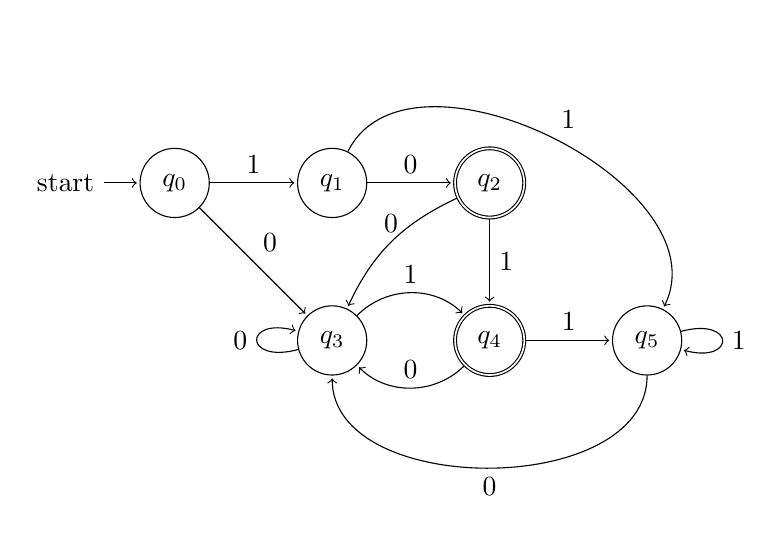
\begin{tikzpicture}[shorten >=1pt,node distance=2cm,on grid,auto]
  \node[state,initial] (q_0)   {$q_0$};
  \node[state] (q_1) [right=of q_0] {$q_1$};
  \node[state,accepting] (q_2) [right=of q_1] {$q_2$};
  \node[state] (q_3) [below=of q_1] {$q_3$};
  \node[state,accepting] (q_4) [right=of q_3] {$q_4$};
  \node[state] (q_5) [right=of q_4] {$q_5$};
  \path[->]
    (q_0) edge  node {0 } (q_3)
          edge node {1} (q_1)
    (q_1) edge node {0} (q_2)
          edge [bend left=90] node {1} (q_5)
    (q_2) edge node {1} (q_4)
          edge [bend right=20] node [above] {0} (q_3)
    (q_3) edge [bend left=45] node  {1} (q_4)
          edge [loop left] node {0} ()
    (q_4) edge node {1} (q_5)
          edge [bend left=45] node [above] {0} (q_3)
    (q_5) edge [bend left=90] node  {0} (q_3)
          edge [loop right] node {1} ();
  \end{tikzpicture}
\end{enumerate}

\vspace{0.2in}

\item \textbf{*Problem 24.11(f,h,w).}
Give DFAs for the following languages, a.k.a.,~computing problems.
\begin{enumerate}[(a)]
\setcounter{enumi}{5}
\item $\mathcal{L}=\{1^{\bullet 2n}01^{\bullet 2k+1}\ |\ n,k\ge 0\}$.
\setcounter{enumi}{7}
\item Strings which begin with 10 and end with 01.
\setcounter{enumi}{22}
\item Strings whose length is divisible by 3.
\end{enumerate}

\vspace{0.2in}

\item \textbf{*Problem 25.7.}
Give a DFA and a CFG for each problem.
\begin{enumerate}[(a)]
\item $\mathcal{L}=\{01^{\bullet n}\ |\ n\ge 0\}$
\item $\mathcal{L}=\{0^{\bullet n}1^{\bullet n}\ |\ 0\le n\le 5\}$
\item $\mathcal{L}=\{$ strings which end in a 1 $\}$.
\end{enumerate}

\end{itemize}

\end{document}
